\begin{figure}[!ht]
%\vspace{-1pt} %takes away some white space before figure
\centering
\begin{subfigure}[b]{1.0\textwidth}
	\centering
	%\includegraphics[clip=true, trim=0pt 240pt 0pt 0pt, width=1.0\textwidth]{figures/evaluationSection/tbi/visualsQualitatively/visualsQualitatively3.png}
	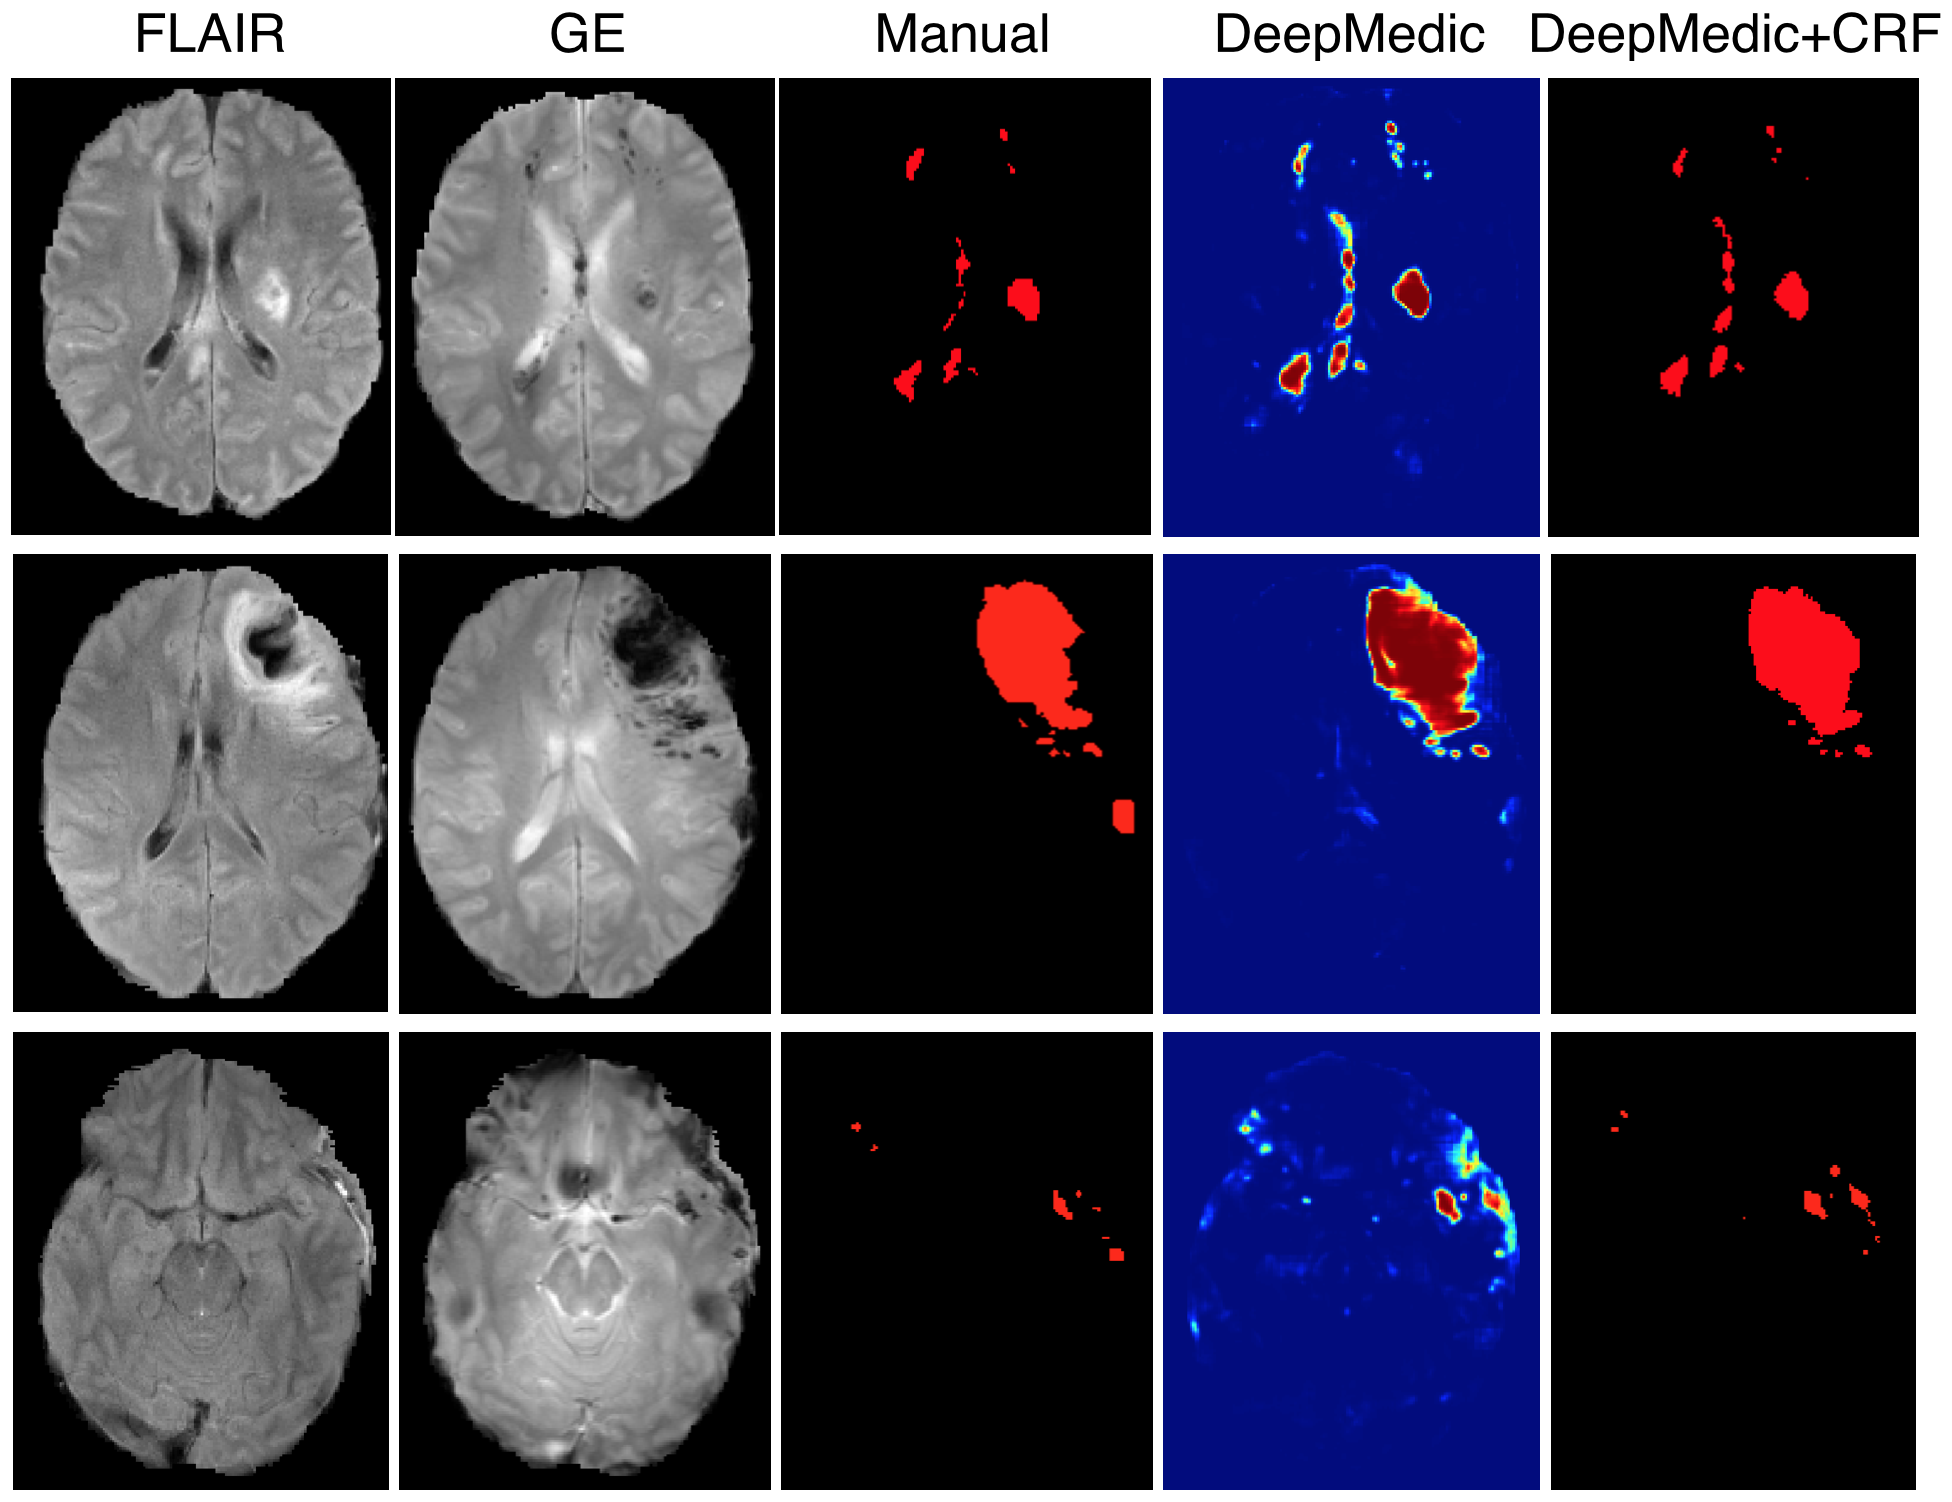
\includegraphics[clip=true, trim=0pt 0pt 0pt 0pt, width=1.0\textwidth]{figures/evaluationSection/tbi/visualsQualitatively/visualsQualitatively4.png}
\end{subfigure}
\vspace{-10pt} %takes away some white space before the caption
\caption{Three examples from the application of our system on the TBI database. It is capable of precise segmentation of both small and large lesions. Second row depicts one of the common mistakes observed. A contusion near the edge of the brain is under-segmented, possibly mistaken for background. Bottom row shows one of the worst cases, representative of the challenges in segmenting TBI. Post-surgical sub-dural debris is mistakenly captured by the brain mask. The network partly segments the abnormality, which is not a celebral lesion of interest.}
\label{fig:evalTbiVisualQuality}
\end{figure}
%\vspace{-1pt} %takes away some white space after figure